%\documentclass[preprint, review, 3p, authoryear]{elsarticle}
\documentclass[10pt, a4paper]{article}

%\usepackage{setspace}
\usepackage[utf8]{inputenc}
\usepackage{amsmath, amssymb, amsthm, bbm}
\usepackage{xcolor}
\usepackage{graphicx}
\usepackage[authoryear]{natbib}
\usepackage{apalike}
\usepackage{relsize}
\usepackage{array}
\usepackage{multirow}
\usepackage{showlabels}
\usepackage{setspace}
\usepackage[normalem]{ulem}
\usepackage{xspace}
\usepackage{svg}
%Add line numbering
%Line numbering can be incorporated by using the lineno package. Add these statements in the preamble:
\usepackage{lineno}
\linenumbers

\DeclareMathOperator*{\argmax}{arg\,max}

\newtheorem{prob}{Problem}
\newtheorem{prop}{Proposition}
\newtheorem{definition}{Definition}

%%%%% bold symbol in math enviornment
\newcommand{\m}[1]{\boldsymbol{#1}}

\newcommand{\fmm}{\textsc{fmm}\xspace}

\title{Merging the components of a finite mixture using  posterior probabilities}
\author{M. Comas-Cufí \and J.A. Martín-Fernández \and G. Mateu-Figueras}

%\doublespacing
\begin{document}

\begin{spacing}{1.9}
%%%%%%% BEGIN SPACING


\pagenumbering{arabic}

\maketitle

\section{Introduction}


% Mixture models
A common approach in parametric cluster analysis assumes data can be modelled by means of a \emph{finite mixture of distributions}, also called \emph{finite mixture model} (\fmm). A \fmm is a probability distribution with probability density function (pdf) defined as the linear combination of pdf from different distributions with same domain $\mathbb{X}$. In general, the pdf $f$ of a \fmm is
\begin{equation}\label{mixt}
f(\;\cdot\; ; \pi_1, \dots, \pi_k, \m\theta_1, \dots, \m\theta_k) = \pi_1 f_1(\;\cdot\; ; \m\theta_1) + \dots + \pi_k f_k(\;\cdot\; ; \m\theta_k),
\end{equation}
where $\m\theta_1, \dots,  \m\theta_k$ are the parameters of the pdf $f_1, \dots, f_k$ respectively and, because $\int_{\mathbb{X}}f = 1$ the restriction $\sum_{\ell = 1}^k \pi_\ell = 1$ holds. The pdf $f_1, \dots, f_k$ are called the \emph{components} of the \fmm, or simply the \emph{mixture components}. \fmm are commonly used in model based clustering [citar Fraley i Raftery, 2002], the clustering approach follows two steps:
\begin{enumerate}
\item to find suitable estimators $\hat{\pi}_1, \dots, \hat{\pi}_k,$ $\hat{\m\theta}_1, \dots, \hat{\m\theta}_k$ of parameters $\pi_1, \dots, \pi_k,$ $\m\theta_1, \dots, \m\theta_k$, and
\item to classify each observation according to the maximum a posteriori criteria, i.e., one observation $\m x_i \in \mathbb{X}$ is classified to cluster $c$ if and only if
\begin{equation}\label{map_criteria}
c=\argmax_{j=1}^k \frac{ \hat{\pi}_j f_j(\m x_i ; \hat{\m\theta}_j) }{\sum_{\ell=1}^k \hat{\pi}_\ell f_\ell(\m x_i ; \hat{\m\theta}_\ell) }.
\end{equation}
\end{enumerate}
Note that in this process, the number of clusters $k$ is fixed in advance. Some strategies have been studied [citar referències].

\cite{lee2004combining,hennig2010methods,baudry2010combining,melnykov2013distribution,pastore2013merging} noted that associating one mixture component to one cluster can be misleading because different mixture components can be not separated enough to be considered as a unique cluster. Instead, they proposed one cluster could be formed by the combination of different mixture components. Therefore, one crucial point of this clustering method is how to decide which components have to be merged, the focus of this article.


We introduce a generic approach to decide which two components should be merged, the approach we introduce depends on two different functions $\lambda$ and $\omega$ which should be defined a priori. For different choices of this functions our approach contains the proposals given by \cite{baudry2010combining}, the DEMP approach introduced by \cite{hennig2010methods} and \cite{longford2014}. Once the criterion for merging component is adopted, from the initial \fmm we can build a hierarchy over the set of components and see which components are more likely to form a single cluster.

The paper is organised as follows: $\dots$


\section{Definitions and notation}

%
A \emph{partition} of $\{1, \dots, k\}$, $\mathcal{P}_s$,  is a set of subsets $I_p$ of $\{1, \dots, k\}$, $1\leq p \leq s$, called $parts$, such that $\bigcup_{I_p \in \mathcal{P}_s} I_p = \{1, \dots, k\}$ and for any two parts $I_a, I_b \in \mathcal{P}_s$ with $a \neq b$, $I_a \cap I_b = \emptyset$ holds. Here it is important to note that for any partition  $\mathcal{P}_s$ the pdf $f$ of a \fmm (Equation~\ref{mixt}) can be rewritten as
\begin{equation}
f = \pi_{I_1} f_{I_1} + \dots + \pi_{I_s} f_{I_s},
\label{mixt_part}
\end{equation}
where $f_{I_p} = \sum_{j \in I_p} \frac{\pi_j}{\pi_{I_p}} f_j(\;\cdot\; ; \m\theta_j)$ and $\pi_{I_p} = \sum_{\ell \in I_p} \pi_\ell$. Moreover, note that using this notation $f_{I_p}$ is also a \fmm.



A \emph{hierarchical sequence of partitions of $\{1,...,k\}$}, is a sequence of partition $\mathcal{P}_1, \dots, \mathcal{P}_k$ verifying that
  
\begin{itemize}
\item $\mathcal{P}_1$ is the one-part partition $\mathcal{P}_1 = \{ \{1, \dots, k\} \}$,
\item for each $s$, $1 <  s \leq k$, $\mathcal{P}_{s}$ has $s$ elements,
\item if a part $I_p \in \mathcal{P}_{s-1}$ then either there is a part $I_a \in \mathcal{P}_{s}$ with $I_p = I_a$ or there are two parts $I_a, I_b \in \mathcal{P}_s$ with $I_p = I_a \cup I_b$, and
\item $\mathcal{P}_k= \{ \{1\},\{2\}, \dots, \{k\} \}$.
\end{itemize}



One can extend Equation~\ref{map_criteria} in terms of partitions. Indeed, let $\rm X = \{\m x_1,\dots, \m x_n\}$ be a sample defined in $\mathbb{X}$. Given a partition $\mathcal{P}_s = \{ I_1, \dots, I_s \}$ the posterior probability of $\m x_i$ being classified to part $I_p\in \mathcal{P}_{s}$ is
\[
\tau_{i I_p} =  \frac{ \hat{\pi}_{I_p} f_{I_p}(\m x_i; \hat{\theta}) }{\sum_{\ell=1}^s \hat{\pi}_{I_\ell} f_{I_p}(\m x_i; \hat{\theta})}.
\]
where $\hat{\pi}_{I_p} = \sum_{\ell \in I_p} \hat{\pi}_\ell$. %From now on, if there is now confusion with parameter $\hat{\theta}$, we are going to use this simplified notation. %\hat{f}_{I_p}(\m x_i) 

For the partition  $\mathcal{P}_s$, we define the posterior probability vector as
\begin{equation}\label{ppv}
\m\tau_{i \mathcal{P}_s} = \left(\tau_{i I_1} , \dots, \tau_{i I_s}  \right).
\end{equation}
Note that because of $\mathcal{P}_s$ is a partition, $\sum_{p=1}^s \tau_{i I_p} = 1$ for $1 \leq i \leq n$.
Moreover, $\m x_i \in \rm X$ is classified to the cluster $c$ if and only if
\begin{equation}\label{cluster_criteria}
c= \argmax_{p=1}^s \{ \tau_{i I_p} \}
\end{equation}

\subsection{Example} \label{example}

Consider following Gaussian mixture with 6 components
\[
f= \sum_{j=1}^6 \pi_j \phi(\;\cdot\; ;  \m\mu_j, \m\Sigma_j)
\]
and parameters given by
{\small \input{tex/partition-example-pars.tex} }

Suppose we want to cluster a random sample coming from mixture $f$. For such purpose, we generate a sample $X$ with 500 observations. In  Figure~\ref{ex_mixture} the sample is represented together with the iso-density curves of the estimated finite mixture.

\begin{figure}[thbp]
\begin{center}
\begin{tabular}{cc}
 %   6 toy mixture
  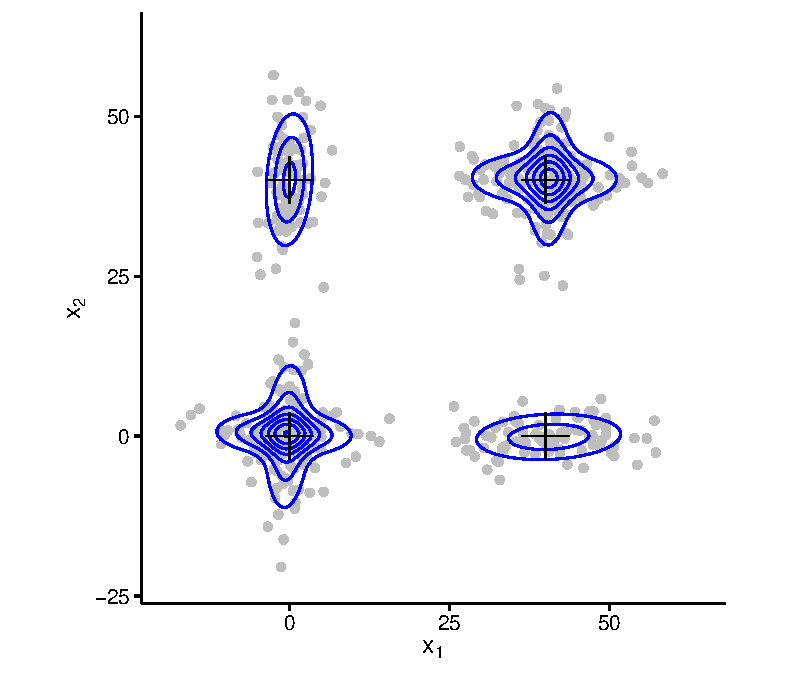
\includegraphics[width=0.7\textwidth]{figures/partition-example-mixture.pdf} \\
 \end{tabular}
 \caption{Density of an adjusted Gaussian mixture with 6 component fitted to data generated from Gaussian mixture. Sample mean estimated of each component is represented by '+'.}\label{ex_mixture}
\end{center}
\end{figure}

Using Equation~\ref{map_criteria} or Equation~\ref{cluster_criteria} with partition $\mathcal{P}_6 = \{ \{1\},\{2\}, \{3\}, \{4\}, \{5\}, \{6\} \}$ yields to a 6 clusters were each component is associated to one cluster as shown in Figure~\ref{ex_one_one}.

\begin{figure}[h]
\begin{center}
\begin{tabular}{cc}
 %   6 toy mixture
  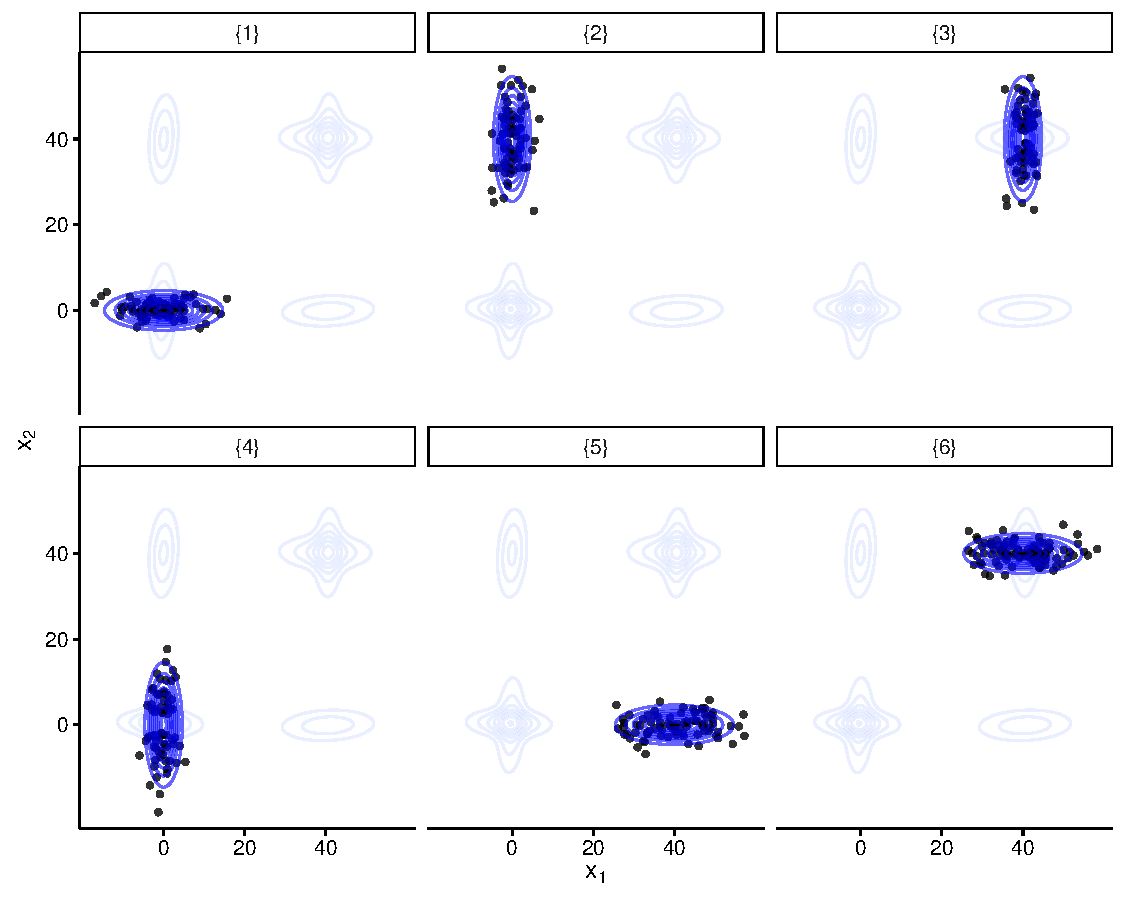
\includegraphics[width=\textwidth]{figures/partition-example-part6.pdf} \\
 \end{tabular}
 \caption{One cluster corresponds to one component}\label{ex_one_one}
\end{center}
\end{figure}

If we consider partition $\mathcal{P}_4 = \{ \{1, 4\},\{2\}, \{5\}, \{6, 3\} \}$, component 1 and 4 define a single cluster, as well as components 3 and 6. In Figure~\ref{ex_two_one} we observe the clustering with the iso-density curves defining each component. Note that in this case, clusters labeled $\{1,4\}$ and $\{6, 3\}$ are modelled with a mixture of two components. Using the notation introduced in this Section, with partition $\mathcal{P}_4$ we are considering components: 
\begin{itemize}
\item $f_{\{1,4\}} = \frac{1}{2} \phi(\;\cdot\; ;  \m\mu_1, \m\Sigma_1) + \frac{1}{2} \phi(\;\cdot\; ;  \m\mu_4, \m\Sigma_4)$, 
\item $f_{\{2\}} = \phi(\;\cdot\; ;  \m\mu_2, \m\Sigma_2)$, 
\item $f_{\{5\}} = \phi(\;\cdot\; ;  \m\mu_5, \m\Sigma_5)$ and
\item $f_{\{6,3\}} = \frac{1}{2} \phi(\;\cdot\; ;  \m\mu_6, \m\Sigma_6) + \frac{1}{2} \phi(\;\cdot\; ;  \m\mu_3, \m\Sigma_3)$.
\end{itemize}

Using Equation~\ref{cluster_criteria} with partition $\mathcal{P}_4$ each observation $x_i$ is clustered to the component more likely to be generated by (see Figure~\ref{ex_two_one}).

\begin{figure}[h]
\begin{center}
\begin{tabular}{cc}
 %   6 toy mixture
  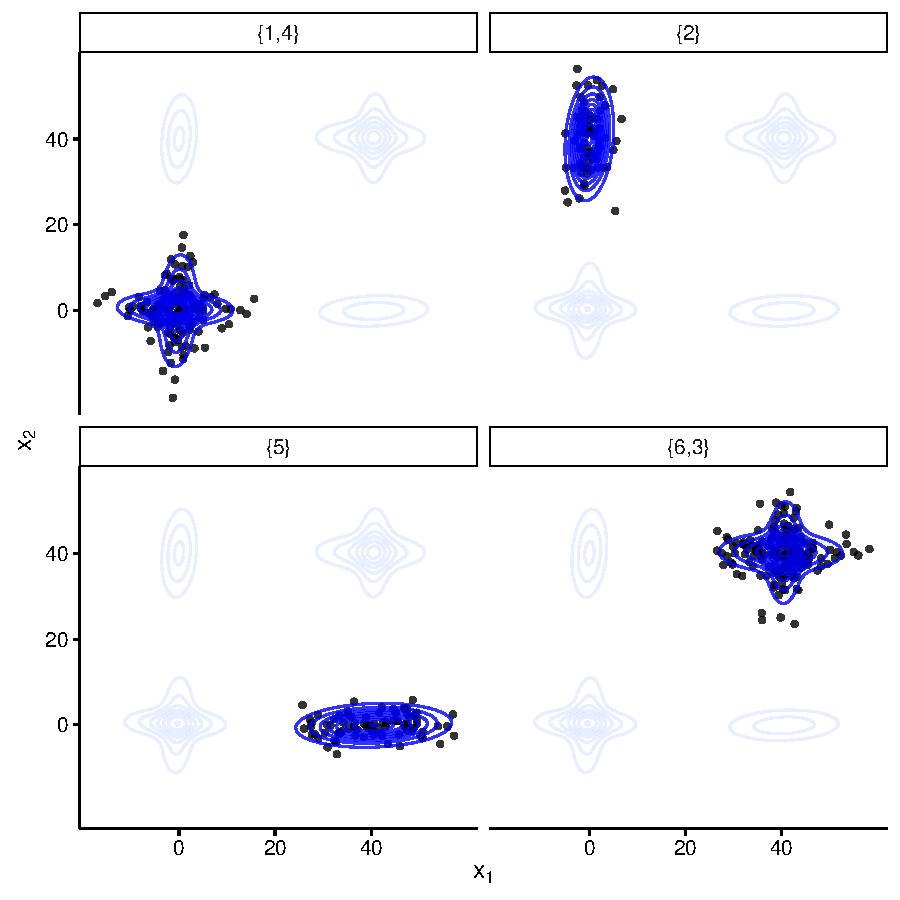
\includegraphics[width=0.65\textwidth]{figures/partition-example-part4.pdf} \\
 \end{tabular}
 \caption{One cluster corresponds to one or more components}\label{ex_two_one}
\end{center}
\end{figure}


A possible hierarchical sequence of partitions of $\{1, 2, 3, 4, 5, 6\}$ is given by the sequence of partition

\begin{equation}
\begin{array}{r c l}
\mathcal{H}(\mathcal{P}) &=& \{ \{\{1, 2, 3, 4, 5, 6\}\}, \\
   & & \;\; \{ \{1, 4, 2, 5\}, \{6, 3\} \},  \\
    & & \;\; \{ \{1, 4, 2\}, \{5\}, \{6, 3\} \}, \\
   & & \;\; \{ \{1, 4\},\{2\}, \{5\}, \{6, 3\} \}, \\
   & & \;\;  \{\{1\},\{2\},\{4\},\{5\},\{6,3\} \},\\
   & &  \;\;  \{\{1\},\{2\},\{3\},\{4\},\{5\},\{6\}\} \}.
\end{array}
\label{hier_ex}
\end{equation}

It is straightforward to verify that if a part $I_p \in \mathcal{P}_{s-1}$ then either there is a part $I_a \in \mathcal{P}_{s}$ with $I_p = I_a$ or there are two parts $I_a, I_b \in \mathcal{P}_s$ with $I_p = I_a \cup I_b$.


\section{Building a hierarchical sequence of partitions using posterior probability vectors}

Let $X = \{\m x_1,\dots,\m x_n \}$ be a sample defined in some sample space $\mathbb{X}$ and let $f$ be a \fmm with $k$ components defined on $\mathbb{X}$ as defined in Equation~\ref{mixt}. Given a partition $\mathcal{P}_s = \{I_1, \dots, I_s\}$, for $i$, $1\leq i \leq n $, let $\m\tau_{i \mathcal{P}_s}$ be the posterior probability vector as defined in Equation~\ref{ppv}. Note that for a fixed $i$, the vector $\m\tau_{i \mathcal{P}_s} =  \left( \tau_{i I_1} , \dots, \tau_{i I_s}  \right)$ is measuring the chances that observation $x_i$ was generated by components $f_{I_p}$, $1 \leq p \leq s$.

In this section we introduce an approach to build a hierarchical sequence of partitions using only the information contained on the posterior probability vectors $\{\m\tau_{i \mathcal{P}_s}\}_{1\leq i \leq n}$ obtained after fitting a \fmm.


Let $\lambda(\m\tau_{i \mathcal{P}_s},  I_a,  I_b)$ be a function measuring how likely is to merge mixture component $\hat{f}_{I_a}$ into mixture component $\hat{f}_{I_b}$ when $\m \tau_{i \mathcal{P}_s}$ is known for an observation $x_i$. Let $\omega(\m\tau_{i \mathcal{P}_s},  I_a,  I_b)$ be a function measuring how reliable is the value $\lambda(\m\tau_{i \mathcal{P}_s},  I_a,  I_b)$.


%For a partition $\mathcal{P}_s = \{ I_1, \dots, I_s\}$ and with functions $\lambda(\m\tau_{i \mathcal{P}_s},  I_a,  I_b)$ and $\omega(\m\tau_{i \mathcal{P}_s},  I_a, I_b)$ fixed, we propose to build a hierarchical sequence of partitions as follows: if $\m\tau_{i \mathcal{P}_s} = \left( \tau_{i I_1} , \dots, \tau_{i I_s}  \right)$ are the posterior probability vectors of observation $x_i$, $1 \leq i \leq n$,  merge those two parts $I_a$ and $I_b$, into one part $I_a \cup I_b$ which maximise

For a given partition $\mathcal{P}_s$ and functions $\lambda$ and $\omega$ fixed we propose to merge those two parts $I_a, I_b \in \mathcal{P}_s$ maximising

\begin{equation}\label{unifying_equation}
S_{\omega, \lambda}( \m\tau_{\mathcal{P}_s},  I_a,  I_b) = \frac{\sum_{i=1}^n \omega(\tau_{i \mathcal{P}_s}, I_a, I_b) \lambda(\tau_{i \mathcal{P}_s}, I_a, I_b)}{\sum_{i=1}^n \omega(\tau_{i \mathcal{P}_s}, I_a) }.
\end{equation}


One can see that the process of starting from partition $\mathcal{P}_k = \{ \{1\}, \dots, \{k\} \}$ and repeatedly maximise Equation~\ref{unifying_equation} yields to a hierarchical sequence of partitions which only depends on the selection of functions $\omega$ and $\lambda$.


\section{Some examples for functions $\omega$ and $\lambda$}

\subsection{Minimising the final entropy}
\label{entropy_section}

The Entropy of a posterior probability vector $\m\tau_{i \mathcal{I}_s} = \left( \hat{\tau}_{i I_1} , \dots, \hat{\tau}_{i I_s}  \right)$ is
\[
\text{Ent}( \m\tau_{i \mathcal{P}_s} ) = \sum_{j=1}^s \tau_{i I_j}  \log(\tau_{i I_j} ).
\]


\cite{baudry2010combining} proposed an algorithm to build a hierarchical sequence of partitions. Starting from partition $\mathcal{P}_s = \{ I_1, \dots, I_s\}$ the algorithm iteratively merges two parts. If we denote $\m\tau_{i \mathcal{P}_s(I_a\cup I_b)}$ the partition obtained after merging part $I_a$ and $I_b$. The two parts $I_a$ and $I_b$ the algorithm merges are those two parts that minimises the overall entropy after merging them, that is the two parts $I_a$ and $I_b$ minimising

\[
\sum_{i=1}^n \text{Ent}( \m\tau_{i \mathcal{P}_s(I_a\cup I_b)} ).
\]


In fact, \cite{baudry2010combining}  argue that equivalent to minimise previous expression is to maximise the difference

\[
\sum_{i=1}^n \text{Ent}( \m\tau_{i \mathcal{P}_s} ) - \text{Ent}( \m\tau_{i \mathcal{P}_s(I_a\cup I_b)} ).
\]

which can be rewritten in terms of $\m\tau_{i \mathcal{I}_s} = \left( \hat{\tau}_{i I_1} , \dots, \hat{\tau}_{i I_s}  \right)$ as

\begin{equation}\label{entropy}
\sum_{i=1}^n  (\tau_{iI_a}+\tau_{iI_b}) \log(\tau_{iI_a} + \tau_{iI_b}) - \left\{ \tau_{iI_a} \log(\tau_{iI_a}) + \tau_{iI_b} \log(\tau_{iI_b}) \right\}.
\end{equation}

The last maximisation problem suggests to define function $\lambda$ as

\[
\lambda(\m\tau_{i \mathcal{P}_s},  I_a,  I_b) =  (\tau_{iI_a}+\tau_{iI_b}) \log(\tau_{iI_a} + \tau_{iI_b}) - \left\{ \tau_{iI_a} \log(\tau_{iI_a}) + \tau_{iI_b} \log(\tau_{iI_b}) \right\}.
\]

which calculates the entropy increment given by each observation. Because in Equation~\ref{entropy} is the sum of $\lambda(\m\tau_{i \mathcal{P}_s},  I_a,  I_b)$ for $1 \leq i \leq n$, to do $S_{\omega, \lambda}( \m\tau_{\mathcal{P}_s},  I_a,  I_b) $ equivalent to the approach presented by \cite{baudry2010combining}, we can define $\omega$ to be constant, for example 

\[
\omega(\m\tau_{i \mathcal{P}_s},  I_a,  I_b) = 1.
\]

Equation~\ref{unifying_equation} takes the form

\[
S_{\omega, \lambda}( \m\tau_{\mathcal{P}_s},  I_a,  I_b) = \frac{1}{n} \sum_{i=1}^n (\tau_{iI_a}+\tau_{iI_b}) \log(\tau_{iI_a} + \tau_{iI_b}) - \left\{ \tau_{iI_a} \log(\tau_{iI_a}) + \tau_{iI_b} \log(\tau_{iI_b}) \right\}
\]


\subsection{Maximising the misclassification probability}
\label{missclassification_section}

A different approach is introduced in \cite{hennig2010methods}. It is proposed to combine the two parts $I_a$ and $I_b$ from $ \mathcal{I}_s$ such that \emph{the probability of classifying an observation generated from component $\hat{f}_{I_a}$ to component $\hat{f}_{I_b}$} is maximum.

To estimate that probability,  \cite{hennig2010methods} suggested to use a consistent estimator, the Directed Estimated misclassification Probabilities (DEMP). Using the notation previously introduced, the estimator is written as

\[
\frac{ \frac{1}{n} \sum_{i=1}^n {\tau_{iI_a} \mathbbm{1}\left( \forall j\; \tau_{i I_{b}} \geq \tau_{iI_j} \right)}}{ \hat{\pi}_{I_a}},
\]

where $\mathbbm{1}\left( \cdot \right)$ is the indicator function. Moreover, because $ \hat{\pi}_{I_a} = \frac{1}{n} \sum_{i=1}^n \tau_{iI_a}$, the estimator can be rewritten in terms of the posterior probability vector as
\begin{equation}\label{demp_criteria}
\frac{ \sum_{i=1}^n {\tau_{iI_a} \mathbbm{1}\left( \forall j\; \tau_{i I_{b}} \geq \tau_{iI_j} \right)}}{\sum_{i=1}^n \tau_{iI_a} }.
\end{equation}

This approach directly suggest to define

\begin{equation}\label{lambda_demp}
\lambda(\m\tau_{i \mathcal{P}_s},  I_a,  I_b) = \mathbbm{1}\left( \forall j\; \tau_{i I_{b}} \geq \tau_{iI_j} \right)
\end{equation}

and

\[
\omega(\m\tau_{i \mathcal{P}_s},  I_a,  I_b) =  \tau_{iI_a}.
\]

A variation of \cite{hennig2010methods} approach is proposed by \cite{longford2014}. Instead of considering function $\lambda$ given by Equation~\ref{lambda_demp} they proposed to measure the chances of confusing $f_{I_b}$ by $f_{I_a}$ with function $\lambda$ given by

\[
\lambda(\m\tau_{i \mathcal{P}_s},  I_a,  I_b) = \frac{\tau_{iI_b}}{\tau_{iI_a} + \tau_{iI_b}},
\]

giving another definition for function function $S_{\omega, \lambda}( \m\tau_{\mathcal{P}_s},  I_a,  I_b)$.


\subsection{Extending function $\omega$}

In Section~\ref{missclassification_section} and \ref{entropy_section} we have seen different approaches to define function $\omega$ and $\lambda$. Concretely, for function $\omega$ we have seen

\begin{itemize}
\item $\omega(\m\tau_{i \mathcal{P}_s},  I_a,  I_b) = 1$ and
\item $\omega(\m\tau_{i \mathcal{P}_s},  I_a,  I_b) = \tau_{iI_a}$.
\end{itemize}

and for function $\lambda$ 

\begin{itemize}
\item $\lambda(\m\tau_{i \mathcal{P}_s},  I_a,  I_b) =  (\tau_{iI_a}+\tau_{iI_b}) \log(\tau_{iI_a} + \tau_{iI_b}) - \left\{ \tau_{iI_a} \log(\tau_{iI_a}) + \tau_{iI_b} \log(\tau_{iI_b}) \right\}$,
\item $\lambda(\m\tau_{i \mathcal{P}_s},  I_a,  I_b) = \mathbbm{1}\left( \forall j\; \tau_{i I_{b}} \geq \tau_{iI_j} \right)$ and
\item $\lambda(\m\tau_{i \mathcal{P}_s},  I_a,  I_b) = \tau_{iI_b} (\tau_{iI_a} + \tau_{iI_b})^{-1}$.
\end{itemize}

The motivation behind function $\omega(\m\tau_{i \mathcal{P}_s},  I_a,  I_b) = \tau_{iI_a}$ is to weight higher those observations close more related to partition $I_a$. A more extremal weighting can be introduced considering only those observation having $ \tau_{iI_a}$ maximum, i.e.

\[
\omega(\m\tau_{i \mathcal{P}_s},  I_a,  I_b) = \mathbbm{1}\left( \forall j\; \tau_{i I_{a}} \geq \tau_{iI_j} \right)
\]

Following the third definition of function $\lambda$, $\lambda(\m\tau_{i \mathcal{P}_s},  I_a,  I_b) = \tau_{iI_b} (\tau_{iI_a} + \tau_{iI_b})^{-1}$, another very simple function measuring how likely is to classify observation into $I_b$ is to consider the posterior probability $\tau_{i I_{b}}$, i.e.

\[
\lambda(\m\tau_{i \mathcal{P}_s},  I_a,  I_b) = \tau_{iI_b}.
\]

\section{The logratio approach}

In Section~\ref{entropy_section} the motivation of function $\lambda$ is that the closer the posterior probability vector are from $(\frac{1}{s}, \dots, \frac{1}{s})$ more similar are components $f_{I_a}$ and $f_{I_b}$. In contrast, in Section~\ref{missclassification_section} function $\lambda$ measures  the probability of classifying an observation to one component $f_{I_b}$ when the observation was generated from another component $f_{I_a}$.

\cite{aitchison1986statistical} presented a series of tools to statistically study samples defined in the Simplex space $\mathcal{S}^d$, i.e $\mathcal{S}^d = \{ (x_1,\dots, x_d) \;|\; x_i > 0 \text{ and } \sum_{i=1}^k x_i = 1 \}$. Later [Geometric approach to statistical analysis on the simplex] was shown that Aitchison approach was equivalent to define an isometry between $\mathcal{S}^d$ and $\mathbb{R}^{d-1}$ in such a way that classical statistical tools can be applied in the later. 

In this section we are interested in different approaches to measure the chances of merging two parts $I_a$ and $I_b$ taking into an account that the posterior probability vector are observations in the Simplex space. In other words we are interested in defining functions $\lambda$ which takes into an account the geometric structure of $\mathcal{S}^d$. We are going to define two new measures, the first ones is motivated by the Entropy notion introduced in \ref{entropy_section}, the second is based on the misclassification definition given in Section~\ref{missclassification_section}.


In Section~\ref{entropy_section}, confusion between components is measured using the notion that the closer the posterior probability vector is from $(\frac{1}{s}, \dots, \frac{1}{s})$ the more confused are the components. We propose to measure the chances of confusing $I_b$ with $I_a$  by measuring how different are $(\frac{\tau_{i I_a}}{\tau_{i I_a} +\tau_{i I_b}}, \frac{\tau_{i I_b}}{\tau_{i I_a} + \tau_{i I_b}})$ from $(\frac{1}{2}, \frac{1}{2})$. That is, we restrict only on the subcomposition formed with the components taking part in the merging process. To measure the difference between these two posterior probability vectors, we use the norm defined in the Simplex space. Doing so, we guarantee subcompositional coherence in this measurement \citep{aitchison1986statistical}. The norm of a posterior probability vector, $\| (\tau_{iI_a}, \tau_{iI_b}) \|$  defined by \cite{aitchison2002simplicial} is 

\[
\lambda(\m\tau_{i \mathcal{P}_s},  I_a,  I_b) = \left\| (\tau_{iI_a}, \tau_{iI_b}) \right\|^2 = \log^2 \left(\frac{ \tau_{iI_b} }{ \tau_{iI_a} }\right).
\]


In Section~\ref{missclassification_section} the notion of confusion between two components $I_a$ and $I_b$ is measured with the probability of \emph{classifying an observation to component $I_b$ when the observation was generated from component $I_a$}. Conditioning that the observation is generated by $I_a$  the approach measures this probability by observing if the observation has been classified to $I_b$, i.e.  measuring the value $\mathbbm{1}\left( \forall j\; \tau_{i I_{b}} \geq \tau_{i I_j} \right)$. Conditioning that the observation is generated by $I_a$ we propose to measure how likely is to classify an observation to $I_b$ when it was generated from $I_a$ by measuring the relative difference between $\tau_{i I_b}$ and $\tau_{i I_a}$, that is 

\[
\lambda(\m\tau_{i \mathcal{P}_s},  I_a,  I_b) = \log( \tau_{i I_b}/\tau_{i I_a}).
\]

\section{Merging components in a mixture of Gaussian distributions}

In Section~\ref{example} we have a sample of 500 observations coming from a mixture with 6 components. 

We have fitted a gaussian mixture. 6 components seems optimum according to BIC criterion. In Figure~\ref{ex_one_one} the scatter plot for each cluster is shown with its corresponding component. That is considering Equation~\ref{map_criteria} or Equation~\ref{cluster_criteria} with partition $\{\{1\}, \{2\}, \{3\}, \{4\}, \{5\}, \{6\}\}$.

Considering $\omega = 1$ and $\lambda = (\tau_{iI_a}+\tau_{iI_b}) \log(\tau_{iI_a} + \tau_{iI_b}) - \left\{ \tau_{iI_a} \log(\tau_{iI_a}) + \tau_{iI_b} \log(\tau_{iI_b}) \right\}$ as the approach proposed by \cite{baudry2010combining} we obtained the sequential hierarchical partition given by Equation~\ref{hier_ex}. If instead of using \cite{baudry2010combining}  approach, we consider  the DEMP approach introduced in \citep{hennig2010methods}, i.e. $\omega = \tau_{i I_a}$ and $\lambda = \mathbbm{1}\left( \forall j\; \tau_{i I_{b}} \geq \tau_{iI_j} \right)$ the sequential hierarchical partition only changes in level 5

\begin{equation}
\begin{array}{r c l}
\mathcal{H}(\mathcal{P}) &=& \{ \{\{1, 2, 3, 4, 5, 6\}\}, \\
   & & \;\; \{ \{1, 4, 2, 5\}, \{6, 3\} \},  \\
    & & \;\; \{ \{1, 4, 2\}, \{5\}, \{6, 3\} \}, \\
   & & \;\; \{ \{1, 4\},\{2\}, \{5\}, \{6, 3\} \}, \\
   & & \;\;  \{\{1, 4\},\{2\}, \{3\},\{5\},\{6\} \},\\
   & &  \;\;  \{\{1\},\{2\},\{3\},\{4\},\{5\},\{6\}\} \}.
\end{array}
\end{equation}

In Figure~\ref{gaussian_Svalues} we can see that using both approaches the value of function $S$ given by equation Equation~\ref{unifying_equation} drops from considering 4 clusters to consider 3 clusters. This reduction suggests that the correct number of clusters is given by 4 clusters.

\begin{figure}[t]
\begin{center}
\begin{tabular}{cc}
  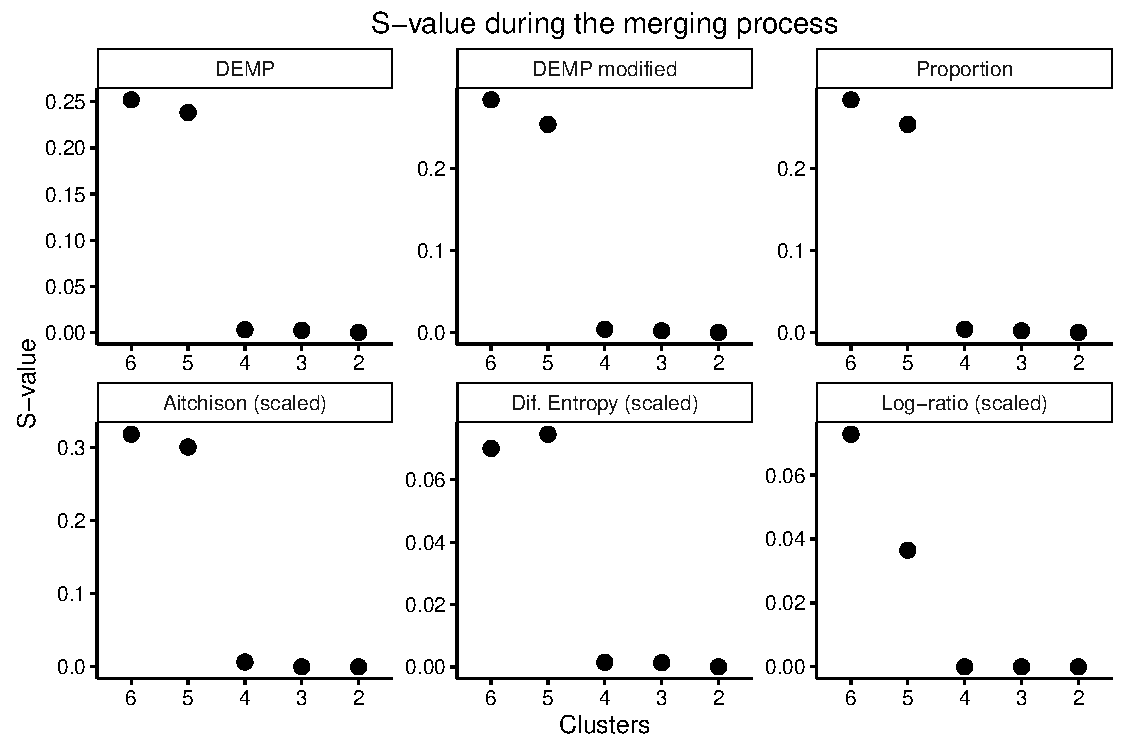
\includegraphics[width=0.85\textwidth]{figures/gaussian_Svalues.pdf} \\
 \end{tabular}
 \caption{S-values obtained using the approaches presented by Baudry et al. and Hennig labeled Entropy and DEMP respectively.}\label{gaussian_Svalues}
\end{center}
\end{figure}

\section{Merging components in a mixture of multinomial distributions}

Merging approaches presented in this article rely on the vector of posterior probabilities this can be calculated by any finite mixture model. In this section we present the scenario where a finite mixture of multinomial is considered.

Pigs dataset can be obtained from package \textsc{zCompositions} R package. The dataset contains a dataset of 29 sows. In different moments the pigs were recorder during 5 minutes and the current activity they were performing was registered. For each pig six locations were considered: straw bed (BED), half in the straw bed (HALF.BED), dunging passage (PASSAGE), half in the dunging passage (HALF.PASS), feeder (FEEDER) and half in the feeder (HALF.FEED). Although the original dataset has 6 different activities, to avoid identifiability problems (Teicher, 1960; Blischke, 1964; Titterington et al., 1985) we eliminate the HALF.PASS, HALF.FEED, HALF.BED which have a very small number of events.

We have used \textsc{mixtools} to fit the mulitinomial mixture. 9 components seems optimum according to BIC criterion. In Figure~\ref{multinomial_mixture} the bar plot for each cluster considering a cluster for each component. That is considering Equation~\ref{map_criteria} or Equation~\ref{cluster_criteria} with partition $\{\{1\}, \{2\}, \{3\}, \{4\}, \{5\}, \{6\}, \{7\}, \{8\}, \{9\} \}$.

\begin{figure}[t]
\begin{center}
\begin{tabular}{cc}
  \includegraphics[width=0.95\textwidth]{figures/multinomial_mixt.pdf} \\
 \end{tabular}
 \caption{Components after adjusting a 9 mixture of multinomial distributions}\label{multinomial_mixture}
\end{center}
\end{figure}

Considering $\omega = \tau_{i I_a}$ and $\lambda = \log^2 \left(\frac{ \tau_{iI_b} }{ \tau_{iI_a} }\right)$ we obtained the sequential hierarchical partition given by


\begin{equation}
\begin{array}{r c l}
\mathcal{H}(\mathcal{P}) &=& \{ \{ \{1,2,3,4,5,6\}\}, \\ 
 & & \;\; \{\{1,2,4\},\{3,5,6\}\}, \\ 
 & & \;\; \{\{1,2,4\},\{3,5\},\{6\}\}, \\ 
 & & \;\; \{\{1,4\},\{2\},\{3,5\},\{6\}\}, \\ 
 & & \;\; \{\{1\},\{2\},\{3,5\},\{4\},\{6\}\}, \\ 
 & & \;\; \{\{1\},\{2\},\{3\},\{4\},\{5\},\{6\} \} \}.
\end{array}
\label{hier_ex_multinomial}
\end{equation}

In next Figure~\ref{multinomial_Svalues} we can see the $S$-value's (Equation~\ref{unifying_equation}) obtained in each step, the drop in $S$-value happens between when considering 2 clusters instead of 3. This fact suggests that when merging from 3 to 2 clusters we are losing valuable information, and therefore, it seems reasonable to stop at 3 clusters.

\begin{figure}[t]
\begin{center}
\begin{tabular}{cc}
  \includegraphics[width=0.65\textwidth]{figures/multinomial_Svalues.pdf} \\
 \end{tabular}
 \caption{S-values obatined}\label{multinomial_Svalues}
\end{center}
\end{figure}

In Figure~\ref{multinomial_clust3} we can see that components 3 and 9 are the first candidates to be merged. They both share the property that the pigs modelled by those two component have higher number in `BED` component and lower number in `FEEDER`.

\begin{figure}[t]
\begin{center}
\begin{tabular}{cc}
  \includegraphics[width=0.95\textwidth]{figures/multinomial_clust3.pdf} \\
 \end{tabular}
 \caption{Components after adjusting a 9 mixture of multinomial distributions}\label{multinomial_clust3}
\end{center}
\end{figure}

\section{Conclusions}

%%% BIBLIOGRAPHY
\newpage

\bibliographystyle{apalike}
\begin{thebibliography}{}

\bibitem[Aitchison, 1986]{aitchison1986statistical}
Aitchison, J. (1986).
\newblock {\em {The Statistical Analysis of Compositional Data}}.
\newblock Monographs on Statistics and Applied Probability. Chapman \& Hall
  Ltd., London (UK).

\bibitem[Aitchison, 2002]{aitchison2002simplicial}
Aitchison, J. (2002).
\newblock {\em {Simplicial inference}}.
\newblock {\em Algebraic Methods in Statistics anb Probability}, 287: 1--22.

\bibitem[Baudry et~al., 2010]{baudry2010combining}
Baudry, J.-P., Raftery, A.~E., Celeux, G., Lo, K., and Gottardo, R. (2010).
\newblock {Combining Mixture Components for Clustering}.

\bibitem[Hennig, 2010]{hennig2010methods}
Hennig, C. (2010).
\newblock {Methods for merging Gaussian mixture components}.
\newblock {\em Advances in Data Analysis and Classification}, 4(1):3--34.

\bibitem[Lee and Cho, 2004]{lee2004combining}
Lee, H.-j. and Cho, S. (2004).
\newblock {Combining Gaussian Mixture Models}.
\newblock In Yang, Z., Yin, H., and Everson, R., editors, {\em Intelligent Data
  Engineering and Automated Learning – IDEAL 2004 SE - 98}, volume 3177 of
  {\em Lecture Notes in Computer Science}, pages 666--671. Springer Berlin
  Heidelberg.

\bibitem[Longford and Bartosova, 2014]{longford2014}
Longford, N.~T. and Bartosova, J. (2014).
\newblock {A confusion index for measuring separation and clustering}.
\newblock {\em Statistical Modelling}, 14(3):229--255.

\bibitem[Meila, 2006]{meila2006comparing}
Meila, M (2006).
\newblock {Comparing clusterings - an information based distance}.
\newblock {\em Journal of Multivariate Analysis}, 98:873--895.

\bibitem[Melnykov, 2013]{melnykov2013distribution}
Melnykov, V. (2013).
\newblock {On the Distribution of Posterior Probabilities in Finite Mixture
  Models with Application in Clustering}.
\newblock {\em Journal of Multivariate Analysis}, 122:175--189.

\bibitem[Pastore and Tonellato, 2013]{pastore2013merging}
Pastore, A. and Tonellato, S.~F. (2013).
\newblock {A Merging Algorithm for Gaussian Mixture Components}.
\newblock {\em SSRN Electronic Journal}, (04).

\bibitem[Melnykov et~al., 2012]{melnikov2012mixsim}
Melnykov, V. and Chen, W.C. and Maitra, R. (2012).
\newblock {MixSim: An R Package for Simulating Data to Study Performance of Clustering Algorithms}.
\newblock {\em Journal of Statistical Software}, 51(12).

\end{thebibliography}

%%%%%%%%%%% END SPACING
\end{spacing}

\end{document}
